\chapter{Codifica}
\label{chap:code}
Gran parte del periodo di stage è stata dedicata allo sviluppo del codice che realizza il sistema di previsione descritto nei capitoli precedenti.
In questo capitolo vengono presentate l’organizzazione della codebase e le principali logiche applicative che la compongono.

\section{Struttura del codice}
\label{chap:codebase}
La struttura delle directory del progetto è organizzata per separare chiaramente i vari componenti e facilitare la navigazione del codice (Figura~\ref{fig:repo-structure}).
Di seguito è riportata una descrizione delle principali cartelle e file presenti nel repository.
\subsection{Root}
\begin{itemize}
    \item \textbf{ErpAI-Forecasting/}: cartella principale del progetto contenente tutto il codice sorgente.
    \begin{itemize}
        \item \textbf{.gitea/}: cartella contenente le configurazioni per l’integrazione continua con Gitea.
        \item \textbf{auth-server/}: modulo di autenticazione.
        \item \textbf{forecasting/}: modulo principale del sistema.
        \item \textbf{duckdb/}: servizio di sincronizzazione dati ERP con scheduler mensile.
        \item \textbf{kong/}: cartella contenente la configurazione del gateway API che espone i servizi interni.
        \item \textbf{openapi/}: servizio che pubblica la documentazione ERP.
        \item \textbf{.env}: variabili d’ambiente.
        \item \textbf{.gitignore}: file di esclusione git.
        \item \textbf{alembic.ini}: configurazione di Alembic per le migrazioni del database.
        \item \textbf{compose.base.yml}: definizione Docker Compose base.
        \item \textbf{compose.yml}: definizione Docker Compose principale.
        \item \textbf{Dockerfile}: build dell’immagine principale.
        \item \textbf{pytest.ini}: configurazioni per i test.
        \item \textbf{README.md}: documentazione di progetto.
    \end{itemize}
\end{itemize}
\subsection{forecasting}
Approfondiamo il modulo di previsione in quanto cuore del sistema e oggetto principale di questo lavoro di tesi.
\begin{itemize}
    \item \textbf{app/}: cartella principale del modulo di previsione.
    \begin{itemize}
        \item \textbf{api/}: cartella che contiene i router FastAPI per gli endpoint REST.
        \item \textbf{db/}: cartella che contiene engine e setup DB locale.
        \item \textbf{dependencies/}: cartella che contiene la configurazione per la dependency injection.
        \item \textbf{models/}: cartella che contiene i modelli Pydantic e SQLModel per payload e tabelle.
        \item \textbf{repositories/}: cartella che contiene le implementazioni del repository pattern per l’accesso ai database esterni.
        \item \textbf{services/}: cartella che contiene le classi che implementano la logica di business e orchestrazione del flusso di previsione.
    \end{itemize}
    \item \textbf{chroma-data/}: cartella che contiene i dati persistenti di Chroma DB.
    \item \textbf{graphs/}: cartella che contiene gli output grafici SHAP generati.
    \item \textbf{migrations/}: cartella che contiene gli script Alembic per la gestione delle migrazioni del database.
    \item \textbf{tests/}: cartella che contiene la suite di test.
    \item \textbf{compose.forecasting.yml}: definizione Docker Compose specifica per il servizio forecasting.
    \item \textbf{Dockerfile}: build dell’immagine del servizio forecasting.
    \item \textbf{requirements.txt}: dipendenze Python.
\end{itemize}

\begin{figure}[H]
    \centering
    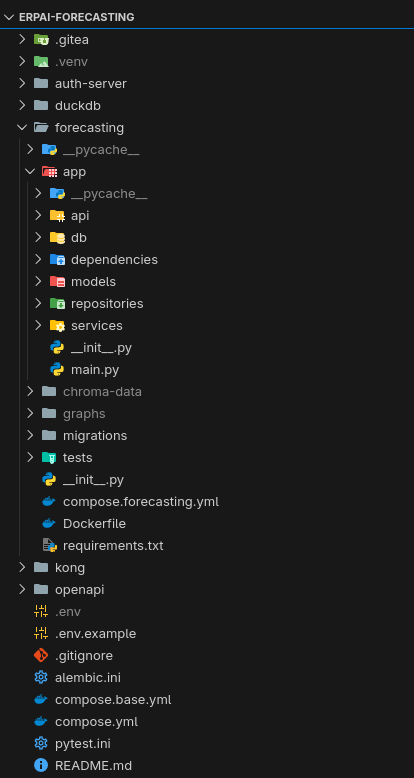
\includegraphics[width=0.6\linewidth]{img/repository.png}
    \caption{Struttura delle directory del progetto.}
    \label{fig:repo-structure}
\end{figure}

\section{Modelli dei dati}
\label{sec:code-models}
Nella cartella \texttt{models/} si trovano i modelli utilizzati per descrivere in modo tipizzato i dati che attraversano l’applicazione: gli schema Pydantic definiscono i payload di richiesta e risposta esposti dalle API FastAPI, mentre i modelli SQLModel rappresentano le tabelle e le relazioni persistite nei database operazionali. Di seguito sono riportati i principali modelli implementati, con una breve descrizione dei campi e il codice di riferimento.
\subsection{Modelli Pydantic}
\subsubsection{Article}
Questo modello definisce e valida un articolo del catalogo prodotti. Ogni \texttt{Article} è composto dai seguenti campi:
\begin{itemize}
    \item \textbf{id}: intero che identifica univocamente l’articolo.
    \item \textbf{name}: stringa con il nome dell’articolo.
    \item \textbf{code}: stringa con il codice identificativo.
    \item \textbf{vat}: numero (float) con l’aliquota IVA associata.
\end{itemize}

\begin{listing}[H]
\inputminted[fontsize=\small, breaklines, breakanywhere=true, linenos=true, bgcolor=gray!10]{python}{code/models/article.py}
\caption{Modello Pydantic \texttt{Article} (\texttt{models/article.py}).}
\label{listing:model-article}
\end{listing}

\subsubsection{Invoice}
Questo modello definisce e valida una fattura con le sue righe di dettaglio. Ogni \texttt{Invoice} include:
\begin{itemize}
    \item \textbf{id}: intero identificativo della fattura.
    \item \textbf{customer}: stringa con l’anagrafica cliente.
    \item \textbf{creating\_date}: data di emissione.
    \item \textbf{expiring\_date}: data di scadenza (opzionale).
    \item \textbf{expected\_shipping\_date} / \textbf{real\_shipping\_date}: date di spedizione prevista/effectiva (opzionali).
    \item \textbf{total}: numero (float) dell’importo totale.
    \item \textbf{articles}: lista di righe articolo (\texttt{ArticleInvoice}).
\end{itemize}
\begin{listing}[H]
\inputminted[fontsize=\small, breaklines, breakanywhere=true, linenos=true, bgcolor=gray!10]{python}{code/models/invoice.py}
\caption{Modello Pydantic \texttt{Invoice} (\texttt{models/invoice.py}).}
\label{listing:model-invoice}
\end{listing}

\subsubsection{Job, JobKind, JobStatus}
Questi modelli definiscono e validano i job di training/forecasting e il loro ciclo di vita. I campi principali sono:
\begin{itemize}
    \item \textbf{job\_id}: stringa identificativa del job.
    \item \textbf{status}: enum con stato corrente (\texttt{queued}, \texttt{running}, \texttt{succeeded}, \texttt{failed}).
    \item \textbf{kind}: enum con il tipo di job (\texttt{training} o \texttt{forecasting}).
    \item \textbf{detail}: stringa opzionale con dettagli/errore.
    \item \textbf{created\_at}, \textbf{started\_at}, \textbf{finished\_at}: timestamp (stringa) di creazione, avvio e fine (opzionali).
\end{itemize}
\begin{listing}[H]
\inputminted[fontsize=\small, breaklines, breakanywhere=true, linenos=true, bgcolor=gray!10]{python}{code/models/job.py}
\caption{Modelli Pydantic \texttt{Job}/\texttt{JobKind}/\texttt{JobStatus} (\texttt{models/job.py}).}
\label{listing:model-job}
\end{listing}

\subsubsection{NotificationEvent}
Questo modello definisce e valida un evento di callback verso ErpAI con stato del job/run:
\begin{itemize}
    \item \textbf{event}: stringa con il tipo di evento notificato.
    \item \textbf{job\_id}: stringa identificativa del job.
    \item \textbf{forecast\_id}: stringa identificativa della run di previsione.
    \item \textbf{status}: stringa con lo stato del job/run.
    \item \textbf{error}: stringa opzionale con il messaggio di errore.
\end{itemize}
\begin{listing}[H]
\inputminted[fontsize=\small, breaklines, breakanywhere=true, linenos=true, bgcolor=gray!10]{python}{code/models/notification.py}
\caption{Modello Pydantic \texttt{NotificationEvent} (\texttt{models/notification.py}).}
\label{listing:model-notification}
\end{listing}

\subsubsection{JWTConfig}
Dataclass che definisce e valida la configurazione JWT:
\begin{itemize}
    \item \textbf{secret\_key}: stringa con la chiave segreta per la firma dei token.
    \item \textbf{algorithm}: stringa con l’algoritmo di firma (es. HS256).
    \item \textbf{expire\_minutes}: intero con la durata di validità dei token in minuti.
\end{itemize}
\begin{listing}[H]
\inputminted[fontsize=\small, breaklines, breakanywhere=true, linenos=true, bgcolor=gray!10]{python}{code/models/jwt_config.py}
\caption{Dataclass \texttt{JWTConfig} (\texttt{models/jwt\_config.py}).}
\label{listing:model-jwt-config}
\end{listing}

\subsubsection{ChromaCollection}
Questo modello definisce e valida un documento indicizzato in Chroma:
\begin{itemize}
    \item \textbf{id}: stringa identificativa del documento.
    \item \textbf{content}: stringa con il testo/descrizione indicizzata.
    \item \textbf{metadata}: dizionario di metadati associati.
    \item \textbf{embedding}: lista di numeri (float) per l’embedding.
\end{itemize}
\begin{listing}[H]
\inputminted[fontsize=\small, breaklines, breakanywhere=true, linenos=true, bgcolor=gray!10]{python}{code/models/chroma_document.py}
\caption{Modello Pydantic \texttt{ChromaCollection} (\texttt{models/chroma\_document.py}).}
\label{listing:model-chroma-document}
\end{listing}

\subsubsection{ShapExplanation}
Questo modello definisce e valida la serializzazione dei valori SHAP:
\begin{itemize}
    \item \textbf{values}: array NumPy di float per i valori SHAP, convertiti in lista in serializzazione.
\end{itemize}
\begin{listing}[H]
\inputminted[fontsize=\small, breaklines, breakanywhere=true, linenos=true, bgcolor=gray!10]{python}{code/models/shap_explanation.py}
\caption{Modello Pydantic \texttt{ShapExplanation} (\texttt{models/shap\_explanation.py}).}
\label{listing:model-shap-explanation}
\end{listing}

\subsubsection{PredictionResult}
Questo modello definisce e valida il payload di risposta con le previsioni future:
\begin{itemize}
    \item \textbf{future\_predictions}: dizionario generico delle previsioni future.
    \item \textbf{MAPE}: numero (float) con la metrica di errore medio percentuale.
\end{itemize}
\begin{listing}[H]
\inputminted[fontsize=\small, breaklines, breakanywhere=true, linenos=true, bgcolor=gray!10]{python}{code/models/prediction_result.py}
\caption{Modello Pydantic \texttt{PredictionResult} (\texttt{models/prediction\_result.py}).}
\label{listing:model-prediction-result}
\end{listing}

\subsubsection{ForecastSearchResult}
Questo modello definisce e valida l’esito di una ricerca semantica su previsioni/spiegazioni:
\begin{itemize}
    \item \textbf{predictions}: lista di stringhe con i risultati previsionali.
    \item \textbf{explanations}: lista di stringhe opzionali con le spiegazioni SHAP.
    \item \textbf{count}: intero con il numero di risultati trovati.
    \item \textbf{fallback}: booleano che indica se è stato usato un percorso di fallback.
    \item \textbf{error}: stringa opzionale con l’eventuale errore riscontrato.
\end{itemize}
\begin{listing}[H]
\inputminted[fontsize=\small, breaklines, breakanywhere=true, linenos=true, bgcolor=gray!10]{python}{code/models/search_result.py}
\caption{Modello Pydantic \texttt{ForecastSearchResult} (\texttt{models/search\_result.py}).}
\label{listing:model-forecast-search-result}
\end{listing}

\subsubsection{ShapExplanation}
Questo modello definisce e valida la serializzazione dei valori SHAP:
\begin{itemize}
    \item \textbf{values}: array NumPy di float per i valori SHAP, convertiti in lista in serializzazione.
\end{itemize}
\begin{listing}[H]
\inputminted[fontsize=\small, breaklines, breakanywhere=true, linenos=true, bgcolor=gray!10]{python}{code/models/shap_explanation.py}
\caption{Modello Pydantic \texttt{ShapExplanation} (\texttt{models/shap\_explanation.py}).}
\label{listing:model-shap-explanation}
\end{listing}

\subsection{Modelli SQLModel}

\subsubsection{XGBoostPrediction}
Questo modello definisce e valida la tabella \texttt{predictions\_xgboost} per le righe previsionali:
\begin{itemize}
    \item \textbf{forecast\_id}: stringa (UUID) di riferimento alla run di previsione.
    \item \textbf{article\_id}: intero identificativo dell’articolo.
    \item \textbf{article\_name}: stringa con il nome dell’articolo.
    \item \textbf{prediction\_date}: data/ora (datetime) della previsione.
    \item \textbf{predicted\_quantity}: numero (float) della quantità stimata.
    \item \textbf{run}: relazione opzionale verso \texttt{ForecastRun} (lato N:1).
\end{itemize}
\begin{listing}[H]
\inputminted[fontsize=\small, breaklines, breakanywhere=true, linenos=true, bgcolor=gray!10]{python}{code/models/prediction.py}
\caption{Modello SQLModel \texttt{XGBoostPrediction} (\texttt{models/prediction.py}).}
\label{listing:model-xgboost-prediction}
\end{listing}

\subsubsection{ForecastRun}
Questo modello definisce e valida la tabella \texttt{forecast\_runs}:
\begin{itemize}
    \item \textbf{id}: stringa UUID identificativa della run.
    \item \textbf{mape}: numero (float) con la metrica di errore della run.
    \item \textbf{created\_at}: timestamp (datetime) di creazione.
    \item \textbf{predictions}: lista di \texttt{XGBoostPrediction} (relazione 1:N).
\end{itemize}
\begin{listing}[H]
\inputminted[fontsize=\small, breaklines, breakanywhere=true, linenos=true, bgcolor=gray!10]{python}{code/models/forecast_run.py}
\caption{Modello SQLModel \texttt{ForecastRun} (\texttt{models/forecast\_run.py}).}
\label{listing:model-forecast-run}
\end{listing}

\subsubsection{JobRun}
Questo modello definisce e valida le run dei job persistite in \texttt{jobs}. I campi principali sono:
\begin{itemize}
    \item \textbf{id}: stringa UUID identificativa della run.
    \item \textbf{kind}: enum \texttt{JobKind} che indica il tipo di job.
    \item \textbf{status}: enum \texttt{JobStatus} con lo stato corrente.
    \item \textbf{detail}: stringa opzionale con dettagli/errore.
    \item \textbf{dataset\_id}: stringa opzionale di riferimento al dataset usato.
    \item \textbf{output\_forecast\_run\_id}: stringa opzionale con la run di previsione prodotta.
\item \textbf{created\_at}: timestamp (datetime) di creazione.
    \item \textbf{started\_at}, \textbf{finished\_at}: timestamp (datetime) di avvio e fine (opzionali).
    \item \textbf{updated\_at}: timestamp (datetime) dell’ultimo aggiornamento.
\end{itemize}
\captionsetup{type=listing, aboveskip=2pt, belowskip=0pt}
\inputminted[fontsize=\small, breaklines, breakanywhere=true, linenos=true, bgcolor=gray!10]{python}{code/models/job_run.py}
\captionof{listing}{Modello \texttt{JobRun} (\texttt{models/job\_run.py}).}
\label{listing:model-job-run}

\subsection{Modello di configurazione XGBoost}
\label{sec:code-dataclass-config}
La configurazione di XGBoost è definita come dataclass per garantire tipizzazione forte e default espliciti. \texttt{XGBoostConfig} raccoglie gli iperparametri chiave:
\begin{itemize}
    \item \texttt{n\_estimators}: numero di alberi; più alberi aumentano la capacità ma anche il rischio di overfitting e il tempo di training.
    \item \texttt{learning\_rate}: shrinkage per ogni passo; valori bassi rendono il training più stabile ma richiedono più iterazioni per convergere.
    \item \texttt{max\_depth}: profondità massima degli alberi; controlla la complessità delle interazioni (profondità elevate catturano non linearità ma aumentano l’overfitting).
    \item \texttt{n\_jobs}: core utilizzati nel training; \texttt{-1} sfrutta tutti i core disponibili.
    \item \texttt{min\_child\_weight}: peso minimo in un nodo figlio; evita nodi con poche osservazioni e migliora la robustezza su dati sparsi.
    \item \texttt{subsample}: frazione di righe usate per ciascun albero; introduce bagging stocastico e riduce la varianza.
    \item \texttt{colsample\_bytree}: frazione di colonne per albero; diminuisce la correlazione tra alberi e aiuta la generalizzazione.
    \item \texttt{reg\_lambda} / \texttt{reg\_alpha}: regolarizzazioni L2/L1 sui pesi; tengono sotto controllo la magnitudine dei coefficienti e prevenono modelli troppo complessi.
    \item \texttt{random\_state}: seme di riproducibilità; rende deterministici split e campionamenti.
    \item \texttt{tree\_method} / \texttt{max\_bin}: algoritmo di costruzione e granularità dell’istogramma; \texttt{hist} con \texttt{max\_bin} regola velocità e approssimazione delle soglie.
    \item \texttt{objective}: funzione obiettivo (regressione \texttt{squarederror}); definisce la loss ottimizzata.
    \item \texttt{eval\_metric}: metrica di valutazione interna (RMSE); guida la diagnostica e l’eventuale early stopping.
    \item \texttt{early\_stopping\_rounds}: round senza miglioramento prima di fermare il training (0 = disabilitato); evita iterazioni inutili a metrica saturata.
    \item \texttt{target\_transform}: trasformazione del target (es. \texttt{log1p}); stabilizza la distribuzione e gestisce valori molto variabili.
    \item \texttt{verbosity}: livello di log del training; controlla il dettaglio dell’output.
\end{itemize}

\captionsetup{type=listing, belowskip=0pt}
\inputminted[fontsize=\small, breaklines, breakanywhere=true, linenos=true, bgcolor=gray!10]{python}{code/services/config/xgboost_config.py}
\captionof{listing}{Configurazione \texttt{XGBoostConfig} (\texttt{services/config/xgboost\_config.py}).}
\label{listing:xgboost-config}

\newpage

\section{Servizi}
\label{sec:code-services}
Nella cartella \texttt{services/} si trovano le classi che implementano la logica di business e orchestrano il flusso di previsione.
\subsection{InvoiceConversionService}
\label{sec:code-invoice-conversion-service}
Il servizio \texttt{InvoiceConversionService} si occupa di leggere \texttt{fact\_invoices} dal database DuckDB e restituire un dataframe Pandas pronto per l’addestramento del modello normalizzando tipi, aggregando le fatture per mese e articolo.
Il metodo principale \texttt{convert\_db\_to\_df} svolge le seguenti operazioni:
\begin{itemize}
    \item Interrogare il database DuckDB per estrarre \texttt{fact\_invoices}.
    \item Convertire le colonne data in formato datetime e normalizzare i tipi numerici.
    \item Aggregare le righe per mese e articolo sommando le quantità.
    \item Restituire un dataframe Pandas ordinato.
\end{itemize}
\captionsetup{type=listing, belowskip=0pt}
\inputminted[fontsize=\small, breaklines, breakanywhere=true, linenos=true, bgcolor=gray!10]{python}{code/services/invoice_conversion_service.py}
\captionof{listing}{Servizio \texttt{InvoiceConversionService}}
\label{listing:invoice-conversion-service}

\subsection{DataFrameService}
\label{sec:code-data-frame-service}
Il servizio \texttt{DataFrameService} seleziona e prepara le feature numeriche per l’addestramento:
\begin{itemize}
    \item legge dal config la colonna data e target;
    \item esclude target, data e \texttt{article\_id} dall’insieme delle feature;
    \item opzionalmente include colonne di prezzo e relative derivate;
    \item offre helper per lo split temporale train/test.
\end{itemize}
\captionsetup{type=listing, belowskip=0pt}
\inputminted[fontsize=\small, breaklines, breakanywhere=true, linenos=true, bgcolor=gray!10]{python}{code/services/data_frame_service.py}
\captionof{listing}{Servizio \texttt{DataFrameService}}
\label{listing:data-frame-service}

\subsection{ForecastingDataService}
\label{sec:code-forecasting-data-service}
Il servizio \texttt{ForecastingDataService} coordina la preparazione dei dati unendo conversione fatture e feature engineering:
\begin{itemize}
    \item carica il dataframe fatture tramite \texttt{InvoiceConversionService};
    \item normalizza/filtra la colonna data, applicando opzionalmente un cutoff temporale;
    \item delega a \texttt{DataFrameService} la creazione delle feature e restituisce dataset, feature e target;
    \item espone un helper per generare righe future autoregressive.
\end{itemize}
\captionsetup{type=listing, belowskip=0pt}
\inputminted[fontsize=\small, breaklines, breakanywhere=true, linenos=true, bgcolor=gray!10]{python}{code/services/forecasting_data_service.py}
\captionof{listing}{Servizio \texttt{ForecastingDataService}}
\label{listing:forecasting-data-service}

\subsection{MetricsService}
\label{sec:code-metrics-service}
La classe \texttt{MetricsService} incapsula le metriche di valutazione personalizzate usate per l’addestramento e la diagnosi del modello XGBoost:
\begin{itemize}
    \item \texttt{mape\_percent}: Mean Absolute Percentage Error (MAPE\%).
    \item \texttt{smape\_percent}: Symmetric MAPE (SMAPE\%).
    \item \texttt{wape\_percent}: Weighted Absolute Percentage Error (WAPE\%).
\end{itemize}
\captionsetup{type=listing, belowskip=0pt}
\inputminted[fontsize=\small, breaklines, breakanywhere=true, linenos=true, bgcolor=gray!10]{python}{code/Services/metrics_service.py}
\captionof{listing}{Servizio \texttt{MetricsService} (\texttt{services/metrics\_service.py}).}
\label{listing:metrics-service}

\subsection{NotificationService}
Il servizio \texttt{NotificationService} invia callback HTTP verso il sistema esterno (Laravel) al termine dei job/run:
\begin{itemize}
    \item estrae le credenziali e gli URL dal \texttt{.env} (\texttt{LARAVEL\_LOGIN\_URL}, \texttt{LARAVEL\_MAIL}, \texttt{LARAVEL\_PASSWORD}, \texttt{LARAVEL\_NOTIFY\_URL});
    \item ottiene un token JWT con una richiesta di login e lo usa per autenticare la chiamata di notifica;
    \item accetta payload \texttt{NotificationEvent} o dizionari e li invia in POST all’endpoint di callback.
\end{itemize}
\captionsetup{type=listing, belowskip=0pt}
\inputminted[fontsize=\small, breaklines, breakanywhere=true, linenos=true, bgcolor=gray!10]{python}{code/Services/notification_service.py}
\captionof{listing}{Servizio \texttt{NotificationService} (\texttt{services/notification\_service.py}).}
\label{listing:notification-service}

\subsection{DataNormalizeService}
\label{sec:code-normalize-service}
Il servizio \texttt{DataNormalizeService} è pensato per rendere le previsioni e le spiegazioni comprensibili al Modulo LLM, trasformando numeri e SHAP in linguaggio naturale e documenti indicizzabili.

Esempi di input/output:
\begin{itemize}
    \item \textbf{Input}: previsioni XGBoost (article\_id, prediction\_date, predicted\_quantity) e valori SHAP per ciascuna riga.
    \item \textbf{Output testo (predizioni)}: frasi come “Per l’articolo A123, il 01 marzo 2025 prevediamo 12.4 unità (finestra 1/3).”
    \item \textbf{Output testo (spiegazioni)}: frasi come “Spiegazione per A123 (marzo 2025): feature prezzo scontato ha aumentato la previsione, stagionalità ha ridotto la previsione.”
    \item \textbf{Documenti embedding}: blocchi di testo con contesto (articolo, periodo, quantità, top driver SHAP) e metadati (article\_id, data, forecast\_window).
\end{itemize}

Questi output alimentano sia la presentazione all’utente, sia la creazione di embedding (ChromaDB) per recupero semantico e interazione con l’LLM.

\subsection{XgboostService}
\label{sec:code-xgboost-service}
La classe \texttt{XgboostService} incapsula configurazione, training e predizione del modello XGBoost:
\begin{itemize}
    \item metriche di valutazione personalizzate gestite dal servizio \texttt{MetricsService} (sez.~\ref{sec:code-metrics-service});
    \item servizio dati per preparare feature e target (\texttt{ForecastingDataService}, sez.~\ref{sec:code-forecasting-data-service});
    \item parametri del modello (\texttt{XGBoostConfig}) per controllare alberi, regolarizzazione e sampling.
\end{itemize}
\paragraph{Inizializzazione.}
Il costruttore crea il regressore XGBoost con gli iperparametri di \texttt{XGBoostConfig}, collega il servizio dati e le metriche e inizializza gli stati interni (feature usate, ultima metrica calcolata).
\captionsetup{type=listing, belowskip=0pt}
\inputminted[fontsize=\small, breaklines, breakanywhere=true, linenos=true, bgcolor=gray!10]{python}{code/services/init/xgboost_service_init.py}
\captionof{listing}{Inizializzazione di \texttt{XGBoostService}}
\label{listing:xgboost-service-init}

Il servizio gestisce due processi principali: \textbf{training} (prepara i dati e addestra il modello) e \textbf{previsione} (genera le quantità future).
\paragraph{Training.}
Recupera i dati dal \texttt{ForecastingDataService} e addestra il modello con \texttt{train\_model} (Listing~\ref{listing:xgboost-train-model}). Il cuore è \texttt{\_\_fit\_model}: imputa i missing (mediana/zero), forza il target a valori non negativi, effettua uno split temporale 80/20, applica l’eventuale \texttt{log1p} sul target e allena XGBoost. Se disponibile un hold-out, calcola il WAPE\% (invertendo la trasformazione) e lo salva in \texttt{\_\_last\_wape} per la diagnostica.
\captionsetup{type=listing, belowskip=0pt}
\inputminted[fontsize=\small, breaklines, breakanywhere=true, linenos=true, bgcolor=gray!10]{python}{code/services/def/xgboost_train_model.py}
\captionof{listing}{Metodo \texttt{train\_model}}
\label{listing:xgboost-train-model}

\paragraph{Previsione.}
Per generare le previsioni (Listing~\ref{listing:xgboost-predict}) il servizio:
\begin{itemize}
    \item riaddestra il modello sui dati disponibili fino al mese prima di \texttt{start\_date};
    \item crea le date future e costruisce le feature in modo autoregressivo;
    \item predice le quantità future e restituisce il \texttt{PredictionResult} con la MAPE stimata, la matrice delle feature future e la lista delle colonne usate.
\end{itemize}
\captionsetup{type=listing, belowskip=0pt}
\inputminted[fontsize=\small, breaklines, breakanywhere=true, linenos=true, bgcolor=gray!10]{python}{code/services/def/xgboost_predict.py}
\captionof{listing}{Metodo \texttt{predict} di \texttt{XGBoostService}}
\label{listing:xgboost-predict}

\subsection{ShapService}
Il servizio \texttt{ShapService} fornisce spiegazioni locali e visualizzazioni delle feature per il modello XGBoost:
\begin{itemize}
    \item \texttt{explain\_prediction} calcola i valori SHAP su un set di input tramite \texttt{TreeExplainer}.
    \item \texttt{generate\_summary\_plot} produce il summary plot principale e restituisce il path salvato.
\end{itemize}
\captionsetup{type=listing, belowskip=0pt}
\inputminted[fontsize=\small, breaklines, breakanywhere=true, linenos=true, bgcolor=gray!10]{python}{code/services/def/shap_explain.py}
\captionof{listing}{Metodo \texttt{explain\_prediction} di \texttt{ShapService}}
\label{listing:shap-explain}
\captionsetup{type=listing, belowskip=0pt}
\inputminted[fontsize=\small, breaklines, breakanywhere=true, linenos=true, bgcolor=gray!10]{python}{code/services/def/shap_summary_plot.py}
\captionof{listing}{Metodo \texttt{generate\_summary\_plot} di \texttt{ShapService}}
\label{listing:shap-summary-plot}
\subsection{ForecastingService}
La classe \texttt{ForecastingService} fa da orchestratore principale per il flusso di previsione.
Il metodo chiave è \texttt{forecast} e coordina l’intero processo di previsione:
\begin{itemize}
    \item invoca \texttt{XGBoostService.predict} per ottenere previsioni future e feature generate;
    \item arricchisce il payload con feature usate, MAPE stimata, data finale;
    \item traduce e prepara le previsioni per salvataggio ed esposizione API;
    \item salva i risultati tramite \texttt{ForecastPersistenceService} su database/ChromaDB;
    \item calcola le spiegazioni SHAP e genera i plot di interpretabilità.
\end{itemize}
\captionsetup{type=listing, belowskip=0pt}
\inputminted[fontsize=\small, breaklines, breakanywhere=true, linenos=true, bgcolor=gray!10]{python}{code/Services/forecasting_service.py}
\captionof{listing}{Metodo \texttt{forecast} di \texttt{ForecastingService}}
\label{listing:forecasting-service}

\section{API Router}
Nella cartella \texttt{api/} si trovano i router FastAPI che espongono gli endpoint REST per interagire con il modulo di previsione, coperti da autenticazione JWT tramite le dipendenze definite nel modulo \texttt{jwt\_dependencies}. Per completezza si include anche il router di autenticazione dell’\texttt{auth-server}, che è un modulo separato rispetto al servizio di forecasting ma fornisce le chiavi pubbliche e i token necessari.

\subsection{Authentication (Auth Server)}
\label{sec:code-api-authentication}
Router dell’\texttt{auth-server}, modulo autonomo che rilascia token JWT e pubblica il JWKS usato dagli altri servizi:
\begin{itemize}
    \item \texttt{GET /.well-known/jwks.json}: restituisce il set di chiavi pubbliche in formato JWKS tramite \texttt{JWKService}.
    \item \texttt{POST /token}: espone la dependency \texttt{jwt\_dependencies.get\_new\_token} per generare un nuovo JWT firmato.
\end{itemize}
\captionsetup{type=listing, belowskip=0pt}
\inputminted[fontsize=\small, breaklines, breakanywhere=true, linenos=true, bgcolor=gray!10]{python}{code/api/authentication.py}
\captionof{listing}{Router di autenticazione (\texttt{api/authentication.py}, modulo \texttt{auth-server})}
\label{listing:api-authentication}

\subsection{JWT}
\label{sec:code-api-jwt}
Router minimale per verificare i token JWT in ingresso:
\begin{itemize}
    \item endpoint \texttt{POST /verify-token} che accetta le credenziali via dependency injection e restituisce un semplice messaggio di conferma.
    \item sfrutta \texttt{jwt\_dependencies.check\_token} per bloccare le richieste non autorizzate.
\end{itemize}
\captionsetup{type=listing, belowskip=0pt}
\inputminted[fontsize=\small, breaklines, breakanywhere=true, linenos=true, bgcolor=gray!10]{python}{code/api/jwt.py}
\captionof{listing}{Router JWT (\texttt{api/jwt.py})}
\label{listing:api-jwt}

\subsection{Forecasting}
\label{sec:code-api-forecasting}
L’endpoint di previsione avvia in background una run di forecasting e restituisce subito l’identificativo del job:
\begin{itemize}
    \item \texttt{POST /forecast}: riceve \texttt{start\_date} e \texttt{periods}, crea un \texttt{Job} di tipo \texttt{forecasting} e imposta l’header \texttt{Location} verso \texttt{/jobs/\{id\}}.
    \item avvia un task asincrono che aggiorna lo stato del job (\texttt{queued} $\rightarrow$ \texttt{running} $\rightarrow$ \texttt{succeeded}/\texttt{failed}), invoca \texttt{ForecastingService.forecast} e invia notifiche esterne tramite \texttt{NotificationService}.
    \item in caso di errore durante il task, marca il job come \texttt{failed} e spedisce una notifica con il dettaglio dell’errore.
\end{itemize}
\captionsetup{type=listing, belowskip=0pt}
\inputminted[fontsize=\small, breaklines, breakanywhere=true, linenos=true, bgcolor=gray!10]{python}{code/api/forecasting.py}
\captionof{listing}{Router di previsione (\texttt{api/forecasting.py})}
\label{listing:api-forecasting}

\subsection{Job}
\label{sec:code-api-job}
Router per interrogare lo stato dei job di training/forecasting:
\begin{itemize}
    \item \texttt{GET /jobs}: ritorna la lista dei job con filtri opzionali \texttt{kind} e \texttt{status}.
    \item \texttt{GET /jobs/\{job\_id\}}: restituisce il singolo job oppure 404 se non esiste.
    \item la logica di persistenza e filtro è delegata a \texttt{JobService}.
\end{itemize}
\captionsetup{type=listing, belowskip=0pt}
\inputminted[fontsize=\small, breaklines, breakanywhere=true, linenos=true, bgcolor=gray!10]{python}{code/api/job.py}
\captionof{listing}{Router dei job (\texttt{api/job.py})}
\label{listing:api-job}

\subsection{ChromaDB}
\label{sec:code-api-chromadb}
Endpoint per la ricerca semantica su previsioni ed embedding SHAP indicizzati in ChromaDB:
\begin{itemize}
    \item \texttt{GET /context}: accetta una domanda naturale (\texttt{question}), il numero di risultati desiderati e, opzionalmente, un \texttt{forecast\_id} per filtrare.
    \item inizializza pigramente un singleton di \texttt{ChromaSearchService}, esegue \texttt{query\_forecast} e restituisce predizioni/spiegazioni rilevanti.
    \item in caso di eccezione solleva un \texttt{HTTPException} 500 con il dettaglio dell’errore.
\end{itemize}
\captionsetup{type=listing, belowskip=0pt}
\inputminted[fontsize=\small, breaklines, breakanywhere=true, linenos=true, bgcolor=gray!10]{python}{code/api/chromadb.py}
\captionof{listing}{Router ChromaDB (\texttt{api/chromadb.py})}
\label{listing:api-chromadb}
